\subsection{Tipologie di utenti}

\begin{itemize}
  \item \textbf{Admin:} ha la capacità di accedere al pannello amministrativo e creare,
        modificare o eliminare tutti i tipi di oggetti all’interno del database,
        può inoltre effettuare ricerche sulle entries del database e filtrare i risultati.

        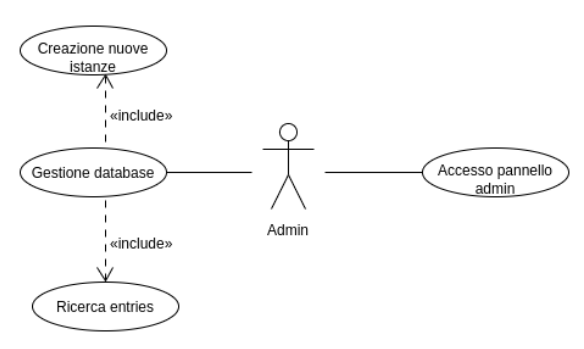
\includegraphics[width=1\linewidth]{images/admin.png}

  \item \textbf{Anonimo:} un utente non registrato ha la possibilità di effettuare ricerche
        e vedere tutti i comics disponibili. Può vedere la pagina dettagliata di un comic, ma non può accedere ai vari capitoli.
        Infine può creare un account.

        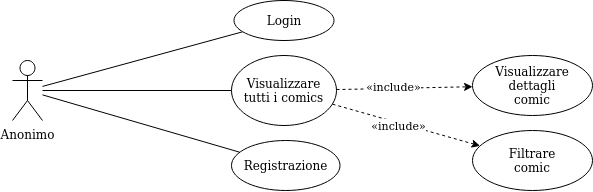
\includegraphics[width=1\linewidth]{images/anonimo.png}

  \item \textbf{Utente:} un utente registrato mantiene tutte le capacità di un utente anonimo.
        \\ L'utente può assegnare un voto da 1 a 10 ad un comic, modificare il suo voto oppure rimuoverlo.
        Può anche salvare il comic nella propria libreria.
        \\In più ha la possibilità di acquistare \textit{coins} che sono una moneta che può essere utilizzata per acquistare
        i vari capitoli di un comic.
        \\ Una volta acquistato un capitolo, l'utente può leggerlo e mettere un \textit{like},
        può lasciare commenti sotto di esso e anche rispondere ad altri commenti.
        \\ Nella pagina riservata all'utente, questo può controllare i propri commenti, i capitoli acquistati,
        i commenti lasciati, i capitoli letti e la propria libreria.
        \\Infine può modificare i propri dati personali, e può anche diventare \textbf{Creator} facendo richiesta.


        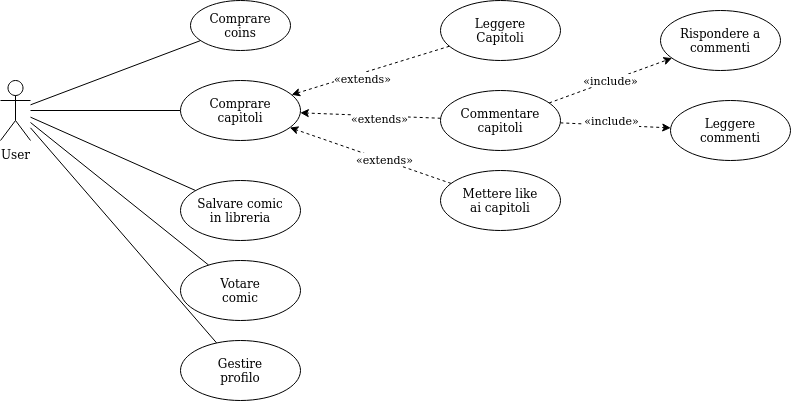
\includegraphics[width=1\linewidth]{images/utente.png}

  \item \textbf{Creator:} un utente con questo ruolo ha la possibilità di creare nuovi comics e caricarne i relativi capitoli.
        \\ Dalla propria pagina utente, può vedere i comics creati e le varie statistiche relative ai vari comics.

        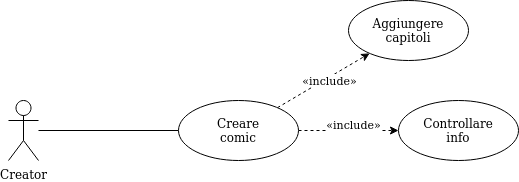
\includegraphics[width=1\linewidth]{images/creatore.png}

\end{itemize}
